\documentclass[10pt]{amsart}

\usepackage{amsmath,amsthm,amssymb,amsfonts}
\usepackage[a4paper]{geometry}
\usepackage{a4wide}
\usepackage{parskip}
\usepackage{graphicx}              % to include figures
\usepackage{mathpazo}
\usepackage{MnSymbol}
\usepackage[T1]{fontenc}
\usepackage[utf8]{inputenc}
\usepackage{enumitem}
\usepackage{hyperref}
\usepackage{color}
\usepackage{xcolor}
\hypersetup{
    colorlinks,
    linkcolor={red!80!black},
    citecolor={blue!80!black},
    urlcolor={blue!80!black}
}
\usepackage{marginnote}
\usepackage{mathrsfs} % fancy font
\usepackage{tikz}          
\usetikzlibrary{matrix,arrows}  % commutative diagrams
\usetikzlibrary{graphs}    % petersen as you may know
\usetikzlibrary{shapes,arrows} % control flow

\usepackage[margin=10pt,font=normalsize,labelfont=bf, labelsep=endash]{caption}
\usepackage{bussproofs} % sequent calculus

\usepackage{listings}
\definecolor{dkgreen}{rgb}{0,0.6,0}
\definecolor{gray}{rgb}{0.5,0.5,0.5}
\definecolor{mauve}{rgb}{0.58,0,0.82}
\lstset{frame=tb,
language=python,
aboveskip=3mm,
belowskip=3mm,
showstringspaces=false,
columns=flexible,
basicstyle={\small\ttfamily},
numbers=none,
numberstyle=\tiny\color{gray},
keywordstyle=\color{blue},
commentstyle=\color{dkgreen},
stringstyle=\color{mauve},
breaklines=true,
breakatwhitespace=true,
tabsize=3,
inputencoding=utf8,
extendedchars=true,
literate={ą}{{\k{a}}}1 {ę}{{\k{e}}}1 {ć}{{\'c}}1 {ł}{{\l}}1 {ń}{{\'n}}1 {ó}{{\'o}}1 {ś}{{\'s}}1 {ż}{{\.z}}1 {ź}{{\'z}}1, 
}

% Define block styles
\tikzstyle{decision} = [diamond, draw, fill=blue!20, 
    text width=4.5em, text badly centered, node distance=3cm, inner sep=0pt]
\tikzstyle{block} = [rectangle, draw, fill=blue!20, 
    text width=5em, text centered, rounded corners, minimum height=4em]
\tikzstyle{line} = [draw, -latex']
\tikzstyle{cloud} = [draw, ellipse,fill=red!20, node distance=3cm,
    minimum height=2em]

\colorlet{myred}{red!80!black}
\colorlet{myblue}{blue!80!black}
\colorlet{mygreen}{green!80!black}

% various theorems, numbered by section
\makeatletter
\def\thm@space@setup{\thm@preskip=4pt
\thm@postskip=2pt}
\makeatother

\newtheorem{theorem}{Theorem}[section]

\newtheorem{corollary}[theorem]{Corollary}
\newtheorem{fact}[theorem]{Fact}

\newtheorem{proposition}[theorem]{Proposition}
\newtheorem{conjecture}[theorem]{Conjecture}

\newtheorem{mainthm}{Theorem}
\renewcommand*{\themainthm}{\Alph{mainthm}}

% lemmas numbered by theorems
\newtheorem{lemma}{Lemma}[theorem]

\theoremstyle{definition} 
\newtheorem{definition}[theorem]{Definition}
\newtheorem{example}[theorem]{Example}
\newtheorem{construction}[theorem]{Construction}
\newtheorem{notation}{Notation}
\newtheorem{remark}[theorem]{Remark}


%############################
%### standard stuff
%############################
\newcommand{\ZZ}{{\mathbb Z}}
\newcommand{\NN}{{\mathbb N}}
\newcommand{\PP}{{\mathbb P}}
\newcommand{\FF}{{\mathbb F}}
\newcommand{\MM}{{\mathbb M}}

\newcommand{\VV}{{\mathbb V}}
\newcommand{\RR}{{\mathbb R}}
\newcommand{\CC}{{\mathbb C}}
\newcommand{\QQ}{{\mathbb Q}}
\newcommand{\EE}{{\mathbb E}}



\newcommand{\cZ}{{\mathcal Z}}
\newcommand{\cY}{{\mathcal Y}}
\newcommand{\cX}{{\mathcal X}}
\newcommand{\cW}{{\mathcal W}}
\newcommand{\cV}{{\mathcal V}}
\newcommand{\cU}{{\mathcal U}}
\newcommand{\cT}{{\mathcal T}}
\newcommand{\cS}{{\mathcal S}}
\newcommand{\cR}{{\mathcal R}}
\newcommand{\cP}{{\mathcal P}}
\newcommand{\cO}{{\mathcal O}}
\newcommand{\cN}{{\mathcal N}}
\newcommand{\cM}{{\mathcal M}}
\newcommand{\cL}{{\mathcal L}}
\newcommand{\cK}{{\mathcal K}}
\newcommand{\cI}{{\mathcal I}}
\newcommand{\cH}{{\mathcal H}}
\newcommand{\cG}{{\mathcal G}}
\newcommand{\cF}{{\mathcal F}}
\newcommand{\cE}{{\mathcal E}}
\newcommand{\cD}{{\mathcal D}}
\newcommand{\cC}{{\mathcal C}}
\newcommand{\cB}{{\mathcal B}}
\newcommand{\cA}{{\mathcal A}}
\newcommand{\cJ}{{\mathcal J}}

\newcommand{\fZ}{{\mathfrak Z}}
\newcommand{\fY}{{\mathfrak Y}}
\newcommand{\fX}{{\mathfrak X}}
\newcommand{\fW}{{\mathfrak W}}
\newcommand{\fV}{{\mathfrak V}}
\newcommand{\fU}{{\mathfrak U}}
\newcommand{\fT}{{\mathfrak T}}
\newcommand{\fS}{{\mathfrak S}}
\newcommand{\fR}{{\mathfrak R}}
\newcommand{\fP}{{\mathfrak P}}
\newcommand{\fO}{{\mathfrak O}}
\newcommand{\fN}{{\mathfrak N}}
\newcommand{\fM}{{\mathfrak M}}
\newcommand{\fL}{{\mathfrak L}}
\newcommand{\fK}{{\mathfrak K}}
\newcommand{\fI}{{\mathfrak I}}
\newcommand{\fH}{{\mathfrak H}}
\newcommand{\fG}{{\mathfrak G}}
\newcommand{\fF}{{\mathfrak F}}
\newcommand{\fE}{{\mathfrak E}}
\newcommand{\fD}{{\mathfrak D}}
\newcommand{\fC}{{\mathfrak C}}
\newcommand{\fB}{{\mathfrak B}}
\newcommand{\fA}{{\mathfrak A}}
\newcommand{\fJ}{{\mathfrak J}}
\newcommand{\fs}{{\mathfrak s}}

\newcommand{\fr}[1]{{\mathfrak{#1}}}

\newcommand{\ra}{\rightarrow}
\newcommand{\la}{\leftarrow}
\newcommand{\rhu}{\rightharpoonup}
\newcommand{\dra}{\dashedrightarrow}


\newcommand{\Ext}{\mathrm{Ext}}
\newcommand{\Hom}{\mathrm{Hom}}
\newcommand{\End}{\mathtrm{End}}
\newcommand{\Spec}{\mathrm{Spec}\,}
\newcommand{\Ker}{\mathrm{ker}}
\newcommand{\Coker}{\mathrm{coker}}
\newcommand{\Image}{\mathrm{im}}

\newcommand{\Proj}{\textrm{Proj}}
\newcommand{\Sym}{\textrm{Sym}}
\newcommand{\Mor}{\mathrm{Mor}}
\newcommand{\Aut}{\mathrm{Aut}}
\newcommand{\Iso}{\mathrm{Iso}}
\newcommand{\Map}{\mathrm{Map}}

\newcommand{\iMor}{\mathcal{M}\mathrm{or}}
\newcommand{\iIso}{\mathcal{I}\mathrm{so}}
\newcommand{\iAut}{\mathcal{A}\mathrm{ut}}

\newcommand{\shHom}{{\mathcal H}om}
\newcommand{\shEnd}{{\mathcal E}nd}


\newcommand{\Set}{\bd{Set}}
\newcommand{\Cat}{\bd{Cat}}
\newcommand{\Fun}{\bd{Fun}}
\newcommand{\Sh}{\bd{Sh}}
\newcommand{\PrSh}{\bd{PrSh}}
\newcommand{\Lrs}{\bd{Lrs}}
\newcommand{\Aff}{\bd{Aff}}
\newcommand{\Rs}{\bd{Rs}}
\newcommand{\Top}{\bd{Top}}
\newcommand{\Sch}{\bd{Sch}}
\newcommand{\Ab}{\bd{Ab}}
\newcommand{\Vect}{\bd{Vect}}
\newcommand{\CRing}{\bd{CRing}}
\newcommand{\Alg}{\bd{Alg}}
\newcommand{\Ban}{\bd{Ban}}
\newcommand{\Comp}{\bd{Comp}}
\newcommand{\sBan}{\bd{sBan}}
\newcommand{\Hdg}{\bd{Hdg}}
\newcommand{\Grp}{\bd{Grp}}
\newcommand{\Lie}{\bd{Lie}}
\newcommand{\Mnd}{\bd{Mnd}}
\newcommand{\GrMod}{\bd{GrMod}}
\newcommand{\Mod}{\bd{Mod}}
\newcommand{\Mon}{\bd{Mon}}
\newcommand{\Qcoh}{\mathfrak{Qcoh}}
\newcommand{\Coh}{\mathfrak{Coh}}
\newcommand{\GrQcoh}{\mathfrak{GrQcoh}}
\newcommand{\ModQcoh}{\mathfrak{ModQcoh}}


\newcommand{\bd}[1]{\mathbf{#1}}  % for bolding symbols
\newcommand{\ol}[1]{\overline{#1}}
\newcommand{\ideal}[1]{\mathfrak{#1}}
\newcommand{\Oplus}{\ensuremath{\vcenter{\hbox{\scalebox{2}{$\oplus$}}}}}

\begin{document}

\title{Hahn-Banach theorem}
\date{}
\maketitle

\section{Introduction}
\noindent
In these notes we study geometric and analytic versions of Hahn-Banach theorem. We find it natural to work in the framework of topological vector spaces thus in the first sections we introduce topological vector spaces over arbitrary fields with absolute value and study their basic properties. Next we prove that all one-dimensional Hausdorff topological spaces are isomorphic. This result is used in the characterization of finite dimensional Hausdorff topological vector spaces over a complete field and is one of the crucial ingredients of Mazur's theorem, which is the main topic of the following section. Next we introduce locally convex topological vector spaces and prove separation of convex sets for these spaces. We use Mazur's theorem to deduce analytic version of Hahn-Banach theorem. In the final section we prove invariant variant of analytic Hahn-Banach theorem.

\section{Fields with absolute values}

\begin{definition}
Let $\mathbb{K}$ be a field and let $|-|:\mathbb{K}\ra \RR_+\cup \{0\}$ be a function such that the following assertions hold.
\begin{enumerate}[label=\textbf{(\arabic*)}, leftmargin=*]
\item $|\alpha| = 0$ if and only if $\alpha = 0$ for every $\alpha \in \mathbb{K}$.
\item $|\alpha\cdot \beta| = |\alpha|\cdot |\beta|$ for every $\alpha,\beta \in \mathbb{K}$.
\item $|\alpha + \beta|\leq |\alpha| + |\beta|$ for every $\alpha,\beta \in \mathbb{K}$.
\end{enumerate}
Then $\mathbb{K}$ together with $|-|$ is \textit{a field with absolute value}.
\end{definition}

\begin{example}\label{example:trivial_absolute_value}
Let $\mathbb{K}$ be a field. Then for each $\alpha \in \mathbb{K}$ define
$$|\alpha| = \begin{cases}
0&\mbox{ if }\alpha = 0\\
1&\mbox{ otherwise}\\
\end{cases}$$
Then $|-|$ is an absolute value on $\mathbb{K}$. It is \textit{the trivial absolute value on $\mathbb{K}$}.
\end{example}
\noindent
Throughout the notes $\mathbb{K}$ is a field with absolute value $|-|$. Note that $|-|$ induces metric 
$$\mathbb{K}\times \mathbb{K} \ni \left(\alpha, \beta\right) \mapsto |\alpha - \beta|\in \RR_+\cup \{0\}$$
In particular, $|-|$ induces topology on $\mathbb{K}$. We always consider $\mathbb{K}$ with this topology.

\begin{fact}\label{fact:trivial_absolute_value_is_the_same_as_discrete_topology}
The topology on a field $\mathbb{K}$ with absolute value is discrete if and only if $|-|$ is trivial.
\end{fact}
\begin{proof}
It suffices to prove that if topology on induced by $|-|$ is discrete, then $|-|$ is trivial. Suppose that there exists $\alpha \in \mathbb{K}$ such that $|\alpha| \not \in \{0,1\}$. Then $\alpha \neq 0$ and 
$$|\alpha|\cdot \bigg|\frac{1}{\alpha}\bigg| = \bigg|\alpha \cdot \frac{1}{\alpha}\bigg| = |1| = 1$$
Hence either 
$$|\alpha| < 1$$ 
or
$$\bigg|\frac{1}{\alpha}\bigg| < 1$$
Without loss of generality we may assume that $0 < |\alpha| < 1$. Then $\{\alpha^n\}_{n\in \NN}$ is a sequence of elements of $\mathbb{K}$ which converges to zero with respect to $|-|$. Thus the topology on $\mathbb{K}$ is not discrete.
\end{proof}

\begin{definition}
The set
$$\mathbb{D} = \big\{\alpha \in \mathbb{K}\,\big|\,|\alpha| \leq 1\big\}$$
is \textit{the closed unit disc in $\mathbb{K}$}.
\end{definition}

\begin{definition}
Suppose that every Cauchy sequence in $\mathbb{K}$ with respect to $|-|$ is convergent, then $\mathbb{K}$ is \textit{a complete field}.   
\end{definition}

\section{Topological vector spaces}
\noindent
In this section we introduce topological vector spaces and study their basic properties.

\begin{definition}
Let $\fX$ be a vector space over $\mathbb{K}$ together with a topology such that the multiplication by scalars $\cdot_{\fX}:\mathbb{K}\times \fX \ra \fX$ and the addition $+_{\fX}:\fX\times \fX\ra \fX$ are continuous. Then $\fX$ is \textit{a topological vector space over $\mathbb{K}$}.
\end{definition}

\begin{fact}\label{fact:topological_vector_subspaces}
Let $\fX$ be a topological vector space over $\mathbb{K}$ and let $\fZ$ be its $\mathbb{K}$-subspace. Then $\fZ$ with subspace topology is a topological vector space over $\mathbb{K}$.
\end{fact}
\begin{proof}
Left for the reader as an exercise.
\end{proof}

\begin{fact}\label{fact:supercircled_open_basis_at_zero}
Let $\fX$ be a topological vector space over $\mathbb{K}$ and let $U$ be an open neighborhood of zero in $\fX$. Then there exists an open neighborhood $W$ of zero in $\fX$ such that $W \subseteq U$ and $W = \mathbb{D}\cdot W$.
\end{fact}
\begin{proof}
Since the multiplication by scalars $\mathbb{K}\times \fX \ra \fX$ is continuous, there exists an open neighborhood $V$ of zero in $\fX$ and a positive real number $r$ such that
$$W = \bigcup_{\alpha\in \mathbb{K},\,|\alpha| \leq r}\alpha \cdot V \subseteq U$$
Then $W$ is an open neighborhood of zero in $\fX$, $W\subseteq U$ and $W = \mathbb{D}\cdot W$.
\end{proof}

\begin{definition}
Let $\fX,\fY$ are topological vector spaces over $\mathbb{K}$. A map $f:\fX\ra \fY$ which is both continuous and $\mathbb{K}$-linear is \textit{a morphism of topological vector spaces over $\mathbb{K}$}.
\end{definition}

\begin{theorem}\label{theorem:quotients_of_topological_vector_spaces}
Let $\fX$ be a topological vector space over $\mathbb{K}$ and let $\fU$ be its $\mathbb{K}$-subspace. Consider the quotient map $q:\fX\twoheadrightarrow \fX/\fU$ in the category of vector spaces over $\mathbb{K}$ and equip $\fX/\fU$ with the quotient topology induced by $q$. Then the following assertions holds.
\begin{enumerate}[label=\emph{\textbf{(\arabic*)}}, leftmargin=*]
\item $q$ is an open map.
\item $\fX/\fU$ is a topological vector space over $\mathbb{K}$ and $q$ is a morphism of topological vector spaces.
\item For every morphism $f:\fX\ra \fY$ of topological vector spaces over $\mathbb{K}$ such that $f\left(\fU\right) = 0$ there exists a unique morphism $p:\fX/\fU\ra \fY$ of topological vector spaces over $\mathbb{K}$ which makes the triangle
\begin{center}
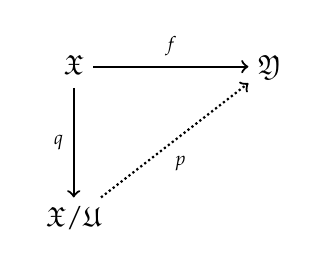
\begin{tikzpicture}
[description/.style={fill=white,inner sep=2pt}]
\matrix (m) [matrix of math nodes, row sep=4em, column sep=5em,text height=1.5ex, text depth=0.25ex] 
{ \fX &  \fY  \\
   \fX/\fU & \\ } ;
\path[->,line width=0.8pt,font=\scriptsize]
(m-1-1) edge node[above] {$ f $} (m-1-2)
(m-1-1) edge node[left] {$ q $} (m-2-1);
\path[densely dotted,->,line width=0.8pt,font=\scriptsize]
(m-2-1) edge node[right = 2pt, below = 2pt] {$ p $} (m-1-2);
\end{tikzpicture}
\end{center}
commutative.
\item $\fU$ is a closed in $\fX$ if and ony if $\fX/\fU$ is a Hausdorff topological space.
\end{enumerate}
\end{theorem}
\noindent
For the proof we need the following result.

\begin{lemma}\label{lemma:Hausdorff_topological_vector_spaces}
Let $\fX$ be a topological vector space over $\mathbb{K}$. Then $\fX$ is Hausdorff if and only if zero subspace of $\fX$ is closed.
\end{lemma}
\begin{proof}[Proof of the lemma]
If $\fX$ is Hausdorff, then each singleton subset of $\fX$ is closed. Hence zero subspace of $\fX$ is closed.\\
Conversely, assume that the singleton of zero in $\fX$ is closed. Pick two distinct points $x_1,x_2 \in \fX$. There exists an open neighborhood $U$ of zero in $\fX$ such that $x_1 - x_2\not \in U$. Since the subtraction $\fX\times \fX\ra \fX$ is continuous, there exists an open neighborhood $V$ of zero in $\fX$ such that $V - V\subseteq U$. If
$$z \in (x_1 + V)\cap (x_2 + V)$$
then $z = x_1 + z_1$ and $z = x_2 + z_2$ for some $z_1,z_2 \in V$. Hence
$$x_1 - x_2 = (z_2 - z_1) \in V - V \subseteq U$$
This is a contradiction with $x_1 - x_2 \not \in U$. Thus
$$\emptyset = (x_1 + V)\cap (x_2 + V)$$
and $\fX$ is Hausdorff.  
\end{proof}

\begin{proof}[Proof of the theorem]
Fix an open subset $U$ of $\fX$, then the set 
$$q^{-1}\left(q\left(U\right)\right) = U + \fU$$
is open. According to the fact that $q:\fX\twoheadrightarrow \fX/\fU$ is a quotient topological map, we infer that $q(U)$ is open in $\fX/\fU$. Hence $q$ is an open map and the proof of \textbf{(1)} is completed.

Since $q$ is open, we derive that $1_{\mathbb{K}}\times q$ and $q\times q$ are open. Since squares
\begin{center}
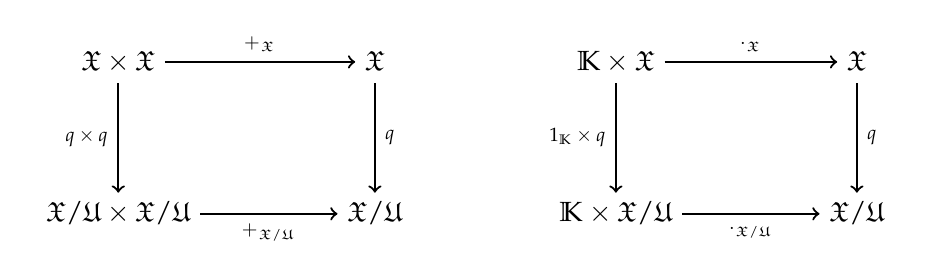
\begin{tikzpicture}
[description/.style={fill=white,inner sep=2pt}]
\matrix (m) [matrix of math nodes, row sep=4em, column sep=5em,text height=1.5ex, text depth=0.25ex] 
{ \fX \times \fX         &  \fX     &  \mathbb{K} \times \fX     &  \fX    \\
\fX/\fU \times \fX/\fU   &  \fX/\fU &  \mathbb{K} \times \fX/\fU &  \fX/\fU  \\ } ;
\path[->,line width=0.8pt,font=\scriptsize]
(m-1-1) edge node[above] {$ +_{\fX} $} (m-1-2)
(m-1-1) edge node[left] {$ q\times q $} (m-2-1)
(m-1-2) edge node[right] {$ q $} (m-2-2)
(m-2-1) edge node[below] {$ +_{\fX/\fU} $} (m-2-2)
(m-1-3) edge node[above] {$ \cdot_{\fX} $} (m-1-4)
(m-1-3) edge node[left] {$ 1_{\mathbb{K}}\times q $} (m-2-3)
(m-1-4) edge node[right] {$ q $} (m-2-4)
(m-2-3) edge node[below] {$ \cdot_{\fX/\fU} $} (m-2-4);
\end{tikzpicture}
\end{center}
are commutative, we deduce that the addition $+_{\fX/\fU}:\fX/\fU \times \fX/\fU \ra \fX/\fU$ and the multiplication of scalars $\cdot_{\fX/\fU}:\mathbb{K}\times \fX/\fU\ra \fX/\fU$ are continuous. Therefore, $\fX/\fU$ is a topological vector space over $\mathbb{K}$. It follows that $q$ is a morphism of topological vector spaces over $\mathbb{K}$ and hence \textbf{(2)} holds.

The assertion \textbf{(3)} describes the universal property which follows easily from \textbf{(2)} and the fact that $q$ is a topological quotient.

For \textbf{(4)} observe that
$$\fU\mbox{ is closed subset of }\fX\,\Leftrightarrow\,\mbox{zero subspace of }\fX/\fU\mbox{ is closed }$$
Thus it suffices to prove that
$$\mbox{ zero subspace of }\fX/\fU\mbox{ is closed }\,\Leftrightarrow\,\fX/\fU\mbox{ is a Hausdorff topological space}$$
but this is a consequence of Lemma \ref{lemma:Hausdorff_topological_vector_spaces}.    
\end{proof}

\section{Complete topological vector spaces}
\noindent
We need some basic results on complete topological vector spaces. For all facts and notions related to filters on topological spaces we refer the reader to \cite{Filters_in_topology}.

\begin{definition}
Let $\fX$ be a topological vector space over $\mathbb{K}$. Suppose that $\cF$ is a proper filter of subsets of $\fX$ such that for every open neighborhood $U$ of zero in $\fX$ there exists $F \in \cF$ such that
$$F - F \subseteq U$$
Then $\cF$ is \textit{a Cauchy filter in $\fX$}.
\end{definition}

\begin{definition}
A topological vector space $\fX$ over $\mathbb{K}$ is \textit{complete} if every Cauchy filter in $\fX$ is convergent.
\end{definition}

\begin{theorem}\label{theorem:complete_subspaces_of_topological_vector_spaces}
Let $\fX$ be a topological vector space over $\mathbb{K}$ and let $\fZ$ be its $\mathbb{K}$-subspace. Consider $\fZ$ as a topological vector space over $\mathbb{K}$ with subspace topology. Then the following assertions hold.
\begin{enumerate}[label=\emph{\textbf{(\arabic*)}}, leftmargin=*]
\item If $\fX$ is complete and $\fZ$ is a closed in $\fX$, then $\fZ$ is complete.
\item If $\fZ$ is complete and $\fX$ is Hausdorff, then $\fZ$ is closed in $\fX$.
\end{enumerate}
\end{theorem}
\begin{proof}
Consider a Cauchy filter $\cF$ in $\fZ$. We define
$$\tilde{\cF} = \big\{\tilde{F}\subseteq \fX\,\big|\,\mbox{ there exists }F\in \cF\mbox{ such that }F\subseteq \tilde{F}\big\}$$
Clearly $\tilde{\cF}$ is a Cauchy filter in $\fX$. Since $\fX$ is complete, we derive that $\tilde{\cF}$ is convergent to some $x$ in $\fX$. This together with definition of $\tilde{\cF}$ show that for every open neighborhood $U$ of zero in $\fX$ there exists $F \in \cF$ such that $F \subseteq x + U$. In particular, for every open neighborhood $U$ of zero in $\fX$ intersection $\left(x + U\right)\cap \fZ$ is nonempty. Since $\fZ$ is closed in $\fX$, it follows that $x \in \fZ$ and $\cF$ is convergent to $x$. Thus $\fZ$ is complete.\\
Suppose now that $\fZ$ is complete. Assume that for some point $x$ in $\fX$ and for every open neighborhood of zero $U$ in $\fX$ intersection $\left(x + U\right) \cap \fZ$ is nonempty. Define
$$\cF = \big\{F \subseteq \fZ\,\big|\,\mbox{ there exists open neighborhood }U\mbox{ of zero in }\fX\mbox{ such that }\left(x + U\right) \cap \fZ \subseteq F\big\}$$
Then $\cF$ is a Cauchy filter in $\fZ$. Since $\fZ$ is complete, $\cF$ is convergent to some point $z$ in $\fZ$. By definition of $\cF$ we have $z \in x + U$ for every open neighborhood $U$ of zero $x$. Since $\fX$ is Hausdorff, it follows that $z$ is identical to $x$. This proves that $\fZ$ is closed in $\fX$.  
\end{proof}

\begin{theorem}\label{theorem:pseudometrizability_completeness_is_determined_by_Cauchy_sequences}
Let $\fX$ be a topological vector space over $\mathbb{K}$. Suppose that there exists a pseudometric $\rho:\fX\times \fX \ra \RR_+\cup \{0\}$ which induces the topology of $\fX$. Then the following assertions hold.
\begin{enumerate}[label=\emph{\textbf{(\roman*)}}, leftmargin=*]
\item $\fX$ is complete.
\item Every Cauchy sequence with respect to $\rho$ is convergent.
\end{enumerate}
\end{theorem}
\begin{proof}
Assume that $\fX$ is complete and $\{x_n\}_{n\in \NN}$ is a Cauchy sequence with respect to $\rho$. Define
$$F_n = \big\{x_k\,\big|\,k\geq n\big\}$$
for every $n\in \NN$ and let 
$$\cF = \big\{F\subseteq \fX\,\big|\,F_n \subseteq F\mbox{ for some }n\in \NN\big\}$$
Since $\{x_n\}_{n\in \NN}$ is a Cauchy sequence with respect to pseudometric $\rho$ which induces topology on $\fX$, we derive that $\cF$ is a Cauchy filter in $\fX$. Hence $\cF$ is convergent to some point of $\fX$. This proves that $\{x_n\}_{n\in \NN}$ is convergent to some point of $\fX$. Hence $\{x_n\}_{n\in \NN}$ is convergent with respect to $\rho$. This completes the proof of $\textbf{(i)}\Rightarrow \textbf{(ii)}$.

Suppose that every Cauchy sequence with respect to $\rho$ is convergent in $\fX$. Consider a Cauchy filter $\cF$ in $\fX$. Since topology of $\fX$ is pseudometrizable, we derive that there exists a countable basis $\{U_n\}_{n\in \NN}$ of open neighborhoods of zero in $\fX$. There exists a decreasing sequence $\{F_n\}$ of elements of $\cF$ such that
$$F_n - F_n\subseteq U_n$$
for each $n\in \NN$. For each $n\in \NN$ let $x_n \in F_n$. Then $\{x_n\}_{n\in \NN}$ is a Cauchy sequence with respect to $\rho$. Hence it is convergent to some point $x$ in $\fX$. Pick an open neighborhood $U$ of zero in $\fX$. Consider open neighborhood $W$ of zero in $\fX$ such that $W + W \subseteq U$. For sufficiently large $n\in \NN$ we have 
$$F_n - F_n \subseteq W,\,x_n - x \in W$$
If $z \in F_n$, then
$$x - z = (x - x_n) + (x_n - z) \in W + (F_n - F_n) \subseteq W + W \subseteq U$$
Hence $F_n \subseteq x + U$. This proves that $\cF$ is convergent to $x$. The implication $\textbf{(ii)}\Rightarrow \textbf{(i)}$ holds.  
\end{proof}

\begin{theorem}\label{theorem:completeness_of_product}
Let $\{\fX_i\}_{i \in I}$ be a family of topological vector space over $\mathbb{K}$. Then the following assertions are equivalent.
\begin{enumerate}[label=\emph{\textbf{(\roman*)}}, leftmargin=*]
\item $\fX_i$ is complete for every $i \in I$.
\item $\prod_{i \in I}\fX_i$ is complete topological vector space over $\mathbb{K}$.
\end{enumerate}
\end{theorem}
\begin{proof}
We denote $\prod_{i\in I}\fX_i$ by $\fX$ and let $pr_i:\fX \ra \fX_i$ be canonical projection on $i$-th axis.

Assume that $\fX_i$ is complete for every $i \in I$. Suppose that $\cF$ is a Cauchy filter in $\fX$. Then $pr_i(\cF)$ is a Cauchy filter in $\fX_i$ for each $i$. Since $\fX_i$ is complete, we derive that $pr_i(\cF)$ is convergent to some point $x_i$ in $\fX_i$. Define $x \in \fX$ by condition $pr_i(x) = x_i$ for each $i \in I$. Then $\cF$ is convergent to $x$. Thus $\fX$ is a complete topological vector space over $\mathbb{K}$.

Suppose now that $\fX$ is complete. Fix $i_0$ in $I$ and consider a Cauchy filter $\cF$ in $\fX_{i_0}$. Define
$$\tilde{F} = \big\{\underbrace{F}_{i_0} \times \underbrace{\{0\}}_{i\neq i_0} \subseteq \fX\,\big|\,F\in \cF\big\}$$
Then $\tilde{\cF}$ is a Cauchy filter in $\fX$. Hence $\tilde{\cF}$ is convergent to some point $x$ in $\fX$. Then $\cF = pr_{i_0}(\tilde{\cF})$ is convergent to $pr_{i_0}(x)$. Thus $\fX_{i_0}$ is complete. Since $i_0$ is arbitrary, we derive that $\fX_i$ is complete for every $i\in I$.
\end{proof}

\begin{corollary}\label{corollary:finite_products_of_copies_of_field_are_complete}
Let $\mathbb{K}$ be a complete field. Topological vector space $\mathbb{K}^n$ over $\mathbb{K}$ is complete for each $n\in \NN$.
\end{corollary}
\begin{proof}
This is a direct consequence of Theorems \ref{theorem:pseudometrizability_completeness_is_determined_by_Cauchy_sequences} and \ref{theorem:completeness_of_product}.
\end{proof}

\section{Finite dimensional topological vector spaces}

\begin{fact}\label{fact:linear_morphisms_from_standard_finite_spaces_are_always_continuous}
Let $\fX$ be a topological vector space over $\mathbb{K}$. Suppose that $f:\mathbb{K}^n \ra \fX$ is a $\mathbb{K}$-linear map for some $n\in \NN$. Then $f$ is continuous.
\end{fact}
\begin{proof}
Let $\{e_1,...,e_n\}$ be the canonical basis of $\mathbb{K}^n$. For every $i$ let $pr_i:\mathbb{K}^n\ra \mathbb{K}$ be the projection onto $i$-th axis and let $m_{i}:\mathbb{K}\ra \fX$ be the composition of the multiplication of scalars $\mathbb{K}\times \fX\ra \fX$ with the continuous embedding $\mathbb{K} \ni \alpha \mapsto \left(\alpha, f(e_i)\right) \in \mathbb{K}\times \fX$. Since $\mathrm{pr}_i$ and $m_{i}$ are continuous for each $i$, we derive that their compositions $m_{i}\cdot pr_i$ are also continuous. According to the fact that the addition $\fX\times \fX\ra \fX$ is continuous, we infer that the sum
$$\sum_{i=1}^n m_{i}\cdot pr_{i}$$
is continuous. This sum is equal to $f$. Thus $f$ is continuous. 
\end{proof}

\begin{theorem}\label{theorem:line_topological_spaces}
Let $\fX$ be a one-dimensional topological vector space over $\mathbb{K}$. Then the following assertions hold.
\begin{enumerate}[label=\emph{\textbf{(\arabic*)}}, leftmargin=*]
\item If $\fX$ is Hausdorff and the absolute value on $\mathbb{K}$ is nontrivial, then every $\mathbb{K}$-linear isomorphism $\fX\ra \mathbb{K}$ is a homeomorphism.
\item If $\fX$ is not Hausdorff, then the topology on $\fX$ is indiscrete.
\end{enumerate}
\end{theorem}
\begin{proof}
Assume that $\fX$ is Hausdorff. Let $f:\fX\ra \mathbb{K}$ be a $\mathbb{K}$-linear isomorphism. The topology on $\mathbb{K}$ is not discrete by Fact \ref{fact:trivial_absolute_value_is_the_same_as_discrete_topology}. Thus for each positive real number $r$ there exists nonzero $\gamma \in \mathbb{K}$ such that $|\gamma| < r$. Consider $x_{\gamma}$ in $\fX$ such that $f(x_{\gamma}) = \gamma$. It is unique element of $\fX$. Since $\fX$ is Hausdorff, by Fact \ref{fact:supercircled_open_basis_at_zero} there exists an open neighborhood $W$ of zero in $\fX$ such that $\mathbb{D}\cdot W = W$ and $x_{\gamma} \not \in W$. Then $\mathbb{D}\cdot f(W) = f(W)$ and $\gamma \not \in f(W)$.
This proves that $f(W)$ is a subset of
$$\big\{\alpha \in \mathbb{K}\,\big|\,|\alpha| < r\big\}$$
Therefore, $f$ is continuous at zero and hence $f$ is continuous. On the other hand map $f^{-1}:\mathbb{K}\ra \fX$ is continuous by Fact \ref{fact:linear_morphisms_from_standard_finite_spaces_are_always_continuous}. This means that $f$ is a homeomorphism.

Suppose now that $\fX$ is not Hausdorff. Theorem \ref{theorem:quotients_of_topological_vector_spaces} implies that zero subspace is not closed in $\fX$. Since in every topological vector space closure of a subspace is a subspace, we derive that $\fX$ is the closure of its zero subspace. This shows that $\fX$ is indiscrete. 
\end{proof}

\begin{example}\label{example:one_dimensional_Hausdorff_space_nonisomorphic_to_line_for_field_with_discrete_abs_value}
Let $\mathbb{K}$ be field of real numbers with trivial absolute value and let $\RR$ be the set of all real numbers with the natural topology.  Then $\RR$ is one-dimensional topological vector space over $\mathbb{K}$, which is not isomorphic to $\mathbb{K}$.
\end{example}

\begin{corollary}\label{corollary:criteria_for_continuity_of_linear_functionals}
Suppose that absolute value on $\mathbb{K}$ is nontrivial. Let $f:\fX \ra \mathbb{K}$ be a $\mathbb{K}$-linear map between topological vector spaces over $\mathbb{K}$. Then the following are equivalent.
\begin{enumerate}[label=\emph{\textbf{(\roman*)}}, leftmargin=*]
\item $f$ is continuous.
\item $\Ker(f)$ is a closed subspace of $\fX$.
\end{enumerate}
\end{corollary}
\begin{proof}
Follows immediately from Theorems \ref{theorem:quotients_of_topological_vector_spaces} and \ref{theorem:line_topological_spaces}.
\end{proof}

\begin{theorem}\label{theorem:uniqueness_of_finite_dimensional_Hausdorff_top_vec_spaces}
Let $\mathbb{K}$ be a complete field with nontrivial absolute value and let $\fX$ be a topological vector space over $\mathbb{K}$. If $\fX$ is Hausdorff and of dimension $n$ over $\mathbb{K}$ for some $n\in \NN$, then $\fX$ is isomorphic with $\mathbb{K}^n$.
\end{theorem}
\begin{proof}
The proof goes on induction by $n\in \NN$. For $n = 0$ it is clear. Suppose that the result holds for $n \in \NN$. Assume that $\fX$ is a Hausdorff topological vector space over $\mathbb{K}$ of dimension $n + 1$. By induction each $n$-dimensional subspace of $\fX$ is isomorphic to $\mathbb{K}^n$ and hence by Corollary \ref{corollary:finite_products_of_copies_of_field_are_complete} it is complete. Thus Theorem \ref{theorem:complete_subspaces_of_topological_vector_spaces} asserts that all $n$-dimensional subspaces are closed in $\fX$. Corollary \ref{corollary:criteria_for_continuity_of_linear_functionals} implies that each $\mathbb{K}$-linear map $f:\fX\ra \mathbb{K}$ is continuous. Therefore, every $\mathbb{K}$-linear map $\Phi:\fX \ra \mathbb{K}^{n+1}$ is continuous. Next $\Phi^{-1}$ is continuous according to Fact \ref{fact:linear_morphisms_from_standard_finite_spaces_are_always_continuous}. Therefore, $\fX$ is isomorphic to $\mathbb{K}^{n+1}$ as a topological vector space over $\mathbb{K}$. The proof is completed.
\end{proof}

\begin{example}\label{example:two_dimensional_top_vec_space_over_rationals_which_is_not_square_of_rationals}
The subspace
$$\QQ + \sqrt{2}\cdot \QQ\subseteq \RR$$
is a two-dimensional Hausdorff topological vector space over $\QQ$. Note that each of its one-dimensional subspaces is dense. Hence
$$\QQ + \sqrt{2}\cdot \QQ \not \cong \QQ\times \QQ$$
as topological vector spaces over $\QQ$.
\end{example}

\begin{corollary}\label{corollary:continuous_map_to_standard_finite_dimensional_is_open}
Let $\mathbb{K}$ be a complete field with nontrivial absolute value and let $\fX$ be a topological vector space over $\mathbb{K}$. Fix a number $n \in \NN$. Then every morphism $f:\fX\ra \mathbb{K}^n$ of topological vector spaces over $\mathbb{K}$ is open.
\end{corollary}
\begin{proof}
Note that $\Ker(f)$ is closed in $\fX$. Hence the quotient map $\fX/\Ker(f)$ is Hausdorff by Theorem \ref{theorem:quotients_of_topological_vector_spaces}. By Theorem \ref{theorem:uniqueness_of_finite_dimensional_Hausdorff_top_vec_spaces} we derive that $\fX/\Ker(f) \cong \mathbb{K}^n$ as topological vector spaces over $\mathbb{K}$. Hence $f$ is the quotient map $q:\fX\ra \fX/\Ker(f)$ followed by an isomorphism $\fX/\Ker(f)\cong \mathbb{K}^n$ of topological vector spaces over $\mathbb{K}$. Theorem \ref{theorem:quotients_of_topological_vector_spaces} implies that $q$ is open. Therefore, $f$ is open.  
\end{proof}

\section{Mazur's theorem}
\noindent
In this section assume that $\mathbb{K}$ is either real numbers field $\RR$ of complex numbers field $\CC$ with usual absolute values.

\begin{theorem}[Mazur]\label{theorem:Mazurs_hyperplane_separation}
Let $\fX$ be a topological vector space over $\mathbb{K}$ and let $U$ be an open and convex subset of $\fX$. Suppose that $\fU$ is a $\mathbb{K}$-subspace of $\fX$ such that $\fU$ does not intersect with $U$. Then there exists a $\mathbb{K}$-linear continuous map $f:\fX\ra \mathbb{K}$ such that $\fU \subseteq \Ker(f)$ and $0 \not \in f(U)$.
\end{theorem}
\noindent
For the proof we need the following result.

\begin{lemma}\label{lemma:two_dimensional_hyperplane_separation}
Let $\fX$ be a two-dimensional Hausdorff topological vector space over $\RR$ and let $U$ be an open and convex subset which does not contain zero of $\fX$. Then there exists one-dimensional subspace $L$ of $\fX$ which does not intersect $U$. 
\end{lemma}
\begin{proof}[Proof of the lemma]
Theorem \ref{theorem:uniqueness_of_finite_dimensional_Hausdorff_top_vec_spaces} implies that we may assume that $\fX$ is $\RR^2$. Consider
$$S^1 = \big\{(x, y)\in \RR^2\,\big|\,x^2 + y^2 = 1\big\}$$
and a retraction $r:\RR^2\setminus \{0\} \ra S^1$ given by formula 
$$r(x, y) = \bigg(\frac{x}{\sqrt{x^2 + y^2}},\frac{y}{\sqrt{x^2 + y^2}}\bigg)$$
Note that $r$ is an open map. Thus $\tilde{U} = r(U)$ is an open subset of $S^1$. Let $i:S^1\ra S^1$ be a homeomorphism given by formula $i(x, y) = (-x, -y)$. Since $U$ is convex and does not contain zero, sets $i(\tilde{U})$ and $\tilde{U}$ have empty intersection. According to the fact that $S^1$ is connected, we deduce that $i(\tilde{U}) \cup \tilde{U}$ is a proper subset of $S^1$. This is the case if and only if there exists $(x, y) \in S^1$ such that $(x, y) \not \in \tilde{U}$ and $(-x, -y) \not \in \tilde{U}$. Then one-dimensional subspace $\RR \cdot (x, y)$ of $\fX$ does not intersect $U$.
\end{proof}

\begin{proof}[Proof of the theorem]
Assume first that $\mathbb{K}$ is $\RR$. By Zorn's lemma there exists maximal $\RR$-subspace $\fZ$ such that $\fU\subseteq \fZ$ and $\fZ$ does not intersect $U$. Since $U$ is open, we derive that $\bd{cl}(\fZ)$ does not intersect $U$. This shows that $\fZ$ is a closed subspace of $\fX$. Now consider the quotient map $q:\fX\twoheadrightarrow \fX/\fZ$. By Theorem \ref{theorem:quotients_of_topological_vector_spaces} space $\fX/\fZ$ is Hausdorff and $q(U)$ is an open set. Moreover, $q(U)$ does not intersect zero and is convex. Suppose that there exists two-dimensional $\RR$-subspace $\fY$ of $\fX/\fZ$. Applying Lemma \ref{lemma:two_dimensional_hyperplane_separation} to $\fY$ and $\fY\cap q(U)$ we deduce that there exists a one-dimensional $\RR$-subspace $L$ of $\fX/\fZ$ such that $L$ does not intersect $q(U)$. Then $q^{-1}(L)$ is $\RR$-subspace of $\fX$ strictly containing $\fZ$ which does not intersect $U$. This is contradiction with maximality of $\fZ$. Thus $\fX/\fZ$ contains no two-dimensional subspaces and hence it is one-dimensional. According to Theorem \ref{theorem:uniqueness_of_finite_dimensional_Hausdorff_top_vec_spaces} we have isomorphism $\phi:\fX/\fZ \ra \RR$ of topological vector spaces over $\RR$. The composition $f = \phi \cdot q$ satisfies the assertion of the theorem and this completes the proof for $\RR$.

Next assume that $\mathbb{K}$ is $\CC$. Since $\fX$ is a topological vector space over $\CC$, it is also topological vector space over $\RR$. Hence there exists an $\RR$-linear continuous map $\tilde{f}:\fX\ra \RR$ such that $\fU \subseteq \Ker(\tilde{f})$ and $0 \not \in \tilde{f}(U)$. Consider $f:\fX\ra \CC$ given by formula
$$f(x) = \tilde{f}(x) - \sqrt{-1}\cdot \tilde{f}\left(\sqrt{-1}\cdot x\right)$$
for $x$ in $\fX$. Then $f$ is a $\CC$-linear continuous map such that $\fU\subseteq \Ker(f)$ and $0\not \in f(U)$.
\end{proof}
\noindent
The result above is often called geometric Hahn-Banach theorem.

\section{Locally convex spaces and separation theorem}
\noindent
In this section assume that $\mathbb{K}$ is either real numbers field $\RR$ of complex numbers field $\CC$ with usual absolute values.

\begin{definition}
Let $\fX$ be a topological vector space over $\mathbb{K}$. Suppose that every open neighborhood of zero in $\fX$ contains an open and convex neighborhood of zero. Then $\fX$ is \textit{a locally convex space over $\mathbb{K}$}.
\end{definition}

\begin{theorem}\label{theorem:separation_in_locally_convex_spaces}
Let $\fX$ be a locally convex space over $\RR$. Suppose that $K$ and $C$ are disjoint, nonempty, convex subsets of $\fX$ such that $K$ is quasi-compact and $C$ is closed in $\fX$. Then there exists a continuous $\RR$-linear map $f:\fX\ra \RR$ and a point $x \in \fX$ such that
$$f\left(K - x\right) \subseteq \RR_-,\,f\left(C - x\right)\subseteq \RR_+$$
\end{theorem}
\begin{proof}
For each $x \in K$ there exists open neighborhood $W_x$ of zero in $\fX$ such that 
$$\left(x + W_x + W_x\right)\cap C = \emptyset$$ 
Since $K$ is quasi-compact, there are $x_1,...,x_n\in K$ such that 
$$K \subseteq \bigcup_{i=1}^n\left(x_i + W_{x_i}\right)$$
Define
$$W = \bigcap_{i=1}^nW_{x_i}$$
Then $W$ is an open neighborhood of zero in $\fX$ such that $\left(K + W\right)\cap C = \emptyset$. Fix now an open and convex neighborhood of zero in $\fX$ such that $V \subseteq W$. Such set exists according to the fact that $\fX$ is locally convex. Note that 
$$\left(K + V\right)\cap C = \emptyset$$
It follows that subset 
$$U = \left(K + V\right) - C$$
of $\fX$ is open, convex and does not contain zero. Invoking Theorem \ref{theorem:Mazurs_hyperplane_separation} we get a continuous $\RR$-linear map $f:\fX \ra \RR$ such that $0 \not \in f\left(U\right)$. Corollary \ref{corollary:continuous_map_to_standard_finite_dimensional_is_open} implies that $f$ is an open map. It follows that $f\left(K + V\right),f\left(C\right)$ are disjoint intervals in $\RR$. Since $f(K)$ is a compact interval contained in an open interval $f(K + V)$, we deduce that there exists $x \in \fX$ such that $f(x)$ is strictly between $f\left(K\right)$ and $f\left(C\right)$. Clearly it is also strictly between $f(K)$ and $f(C)$. Thus $f(K - x)$ and $f(C - x)$ are strictly separated by zero in $\RR$. Without loss of generality we may assume that $f(K - x) \subseteq \RR_-$ and $f(C - x)\subseteq \RR_+$.
\end{proof}

\section{Analytic Hahn-Banach theorem}

\begin{definition}
Let $\fX$ be a vector space over $\RR$ and let $p:\fX\ra \RR$ be a map. Suppose that
$$p(x_1 + x_2)\leq p(x_1) + p(x_2)$$
for all $x_1,x_2\in \fX$ and 
$$p(r\cdot x) = r\cdot p(x)$$
for each $x\in \fX$ and each $r\in \RR_+$. Then $p$ is \textit{a sublinear map}.
\end{definition}

\begin{theorem}[Hahn-Banach]\label{theorem:Hahn_Banach_real_case}
Let $\fX$ be a vector space over $\RR$ and let $p:\fX\ra \RR$ be a sublinear map. Suppose that $\fU$ is an $\RR$-subspace of $\fX$ and $f:\fU\ra \RR$ is an $\RR$-linear map such that $f(x) \leq p(x)$ for every $x$ in $\fU$. Then there exists an $\RR$-linear map $\tilde{f}:\fX \ra \RR$ such that $\tilde{f} \leq p$ and $\tilde{f}_{\mid \fU} = f$. 
\end{theorem}
\noindent
We need the following result, which shows that each sublinear map give rise to a seminorm.

\begin{lemma}\label{lemma:sublinear_induces_seminorm_and_is_continuous_with_respect_to_it}
Let $\fX$ be a vector space over $\RR$ and let $p:\fX \ra \RR$ be a sublinear map. Consider $q:\fX \ra \RR$ given by formula
$$q(x) = \max\{p(x),p(-x)\}$$
for $x \in \fX$. Then $q$ is a seminorm on $\fX$ and $p$ is continuous with respect to $q$. 
\end{lemma}
\begin{proof}[Proof of the lemma]
Note that $q$ is a sublinear map. Since 
$$0\leq p(x) + p(-x)$$
for $x \in \fX$, we derive that the image of $q$ is $\RR_+\cup \{0\}$. Moreover, $q(x) = q(-x)$ for each $x$ in $\fX$. Therefore, $q$ is a seminorm on $\fX$. Observe that
$$|p(x_1) - p(x_2)|\leq q(x_1 - x_2)$$
and hence $p$ is continuous with respect to the topology induced by $q$ on $\fX$.
\end{proof}

\begin{proof}[Proof of the theorem]
By Lemma \ref{lemma:sublinear_induces_seminorm_and_is_continuous_with_respect_to_it} we may assume that $\fX$ is a topological vector space over $\RR$ and $p$ is a continuous map on $\fX$. Define
$$U = \big\{(x,r)\in \fX\times \RR\,\big|\,p(x) < r\big\},\,\fZ = \big\{(x,f(x))\in \fX\times \RR\,\big|\,x\in \fU\big\}$$ 
It follows that $U$ is a convex open subset of $\fX\times \RR$ and $\fZ$ is an $\RR$-subspace of $\fX\times \RR$ such that $U \cap \fZ = \emptyset$. By Theorem \ref{theorem:Mazurs_hyperplane_separation} there exists a codimension one $\RR$-linear subspace $\fM$ of $\fX\times \RR$ such that $\fZ \subseteq \fM$ and $U\cap \fM = \emptyset$. Let $\pi$ be the projection $\fX\times \RR\ra \fX$. It follows from the properties of $\fM$, that $\pi_{\mid \fM}:\fW\ra \fX$ is an $\RR$-linear isomorphism. Hence there exists an $\RR$-linear map $\tilde{f}:\fX \ra \RR$ such that 
$$\fM = \big\{(x,\tilde{f}(x))\in \fX\times \RR\,\big|\,x \in \fX\big\}$$
Since $\fZ \subseteq \fM$, we deduce that $\tilde{f}_{\mid \fU} = f$. According to $U\cap \fW = \emptyset$, we have $\tilde{f} \leq p$. This completes the proof.
\end{proof}

\section{Invariant Hahn-Banach theorem}
\noindent
In this section we prove invariant version of Hahn-Banach theorem. This theorem appears implicitly in \cite[Chapitre II, \S3]{banach1979theorieoperationslineaires} and is related to the previous Banach's manuscript \cite{banach1923problemelameasure} in which the author shows the existence of translation invariant finitely additive extension of Lebesgue measure on real line.

\begin{definition}
Let $\fX$ be a vector space over $\RR$ and let $\cG$ be a semigroup of $\RR$-linear endomorphisms of $\fX$. An $\RR$-linear subspace $\fU$ is \textit{$\fG$-invariant} if $g\left(\fU\right)\subseteq \fU$ for every $g\in \cG$.
\end{definition}

\begin{example}\label{example:whole_space_is_invariant}
Let $\fX$ be a vector space over $\RR$ and let $\cG$ be a semigroup of $\RR$-linear endomorphisms of $\fX$. Then by obvious reasons $\fX$ is $\cG$-invariant subspace.
\end{example}

\begin{definition}
Let $\fX$ be a vector space over $\RR$, let $\cG$ be a semigroup of $\RR$-linear endomorphisms of $\fX$ and let $\fU$ be a $\cG$-invariant subspace of $\fX$. An $\RR$-linear map $f:\fU\ra \RR$ is \textit{$\cG$-invariant} if
$$f\left(g(x)\right) = f(x)$$
for every $x\in \fU$ and $g\in \cG$.
\end{definition}
\noindent
Now we are ready to state the result.

\begin{theorem}\label{theorem:invariant_Hahn_Banach}
Let $\fX$ be a vector space over $\RR$ and let $\cG$ be a commutative semigroup of $\RR$-linear endomorphisms of $\fX$. Suppose that $p:\fX\ra \RR$ is a sublinear map such that
$$p\left(g(x)\right) \leq p(x)$$
for every $x \in \fX$ and $g \in \cG$. If $\fU$ is a $\cG$-invariant subspace of $\fX$ and $f:\fU\ra \RR$ is an $\RR$-linear and $\cG$-invariant map such that $f(x)\leq p(x)$ for all $x\in \fU$, then there exists an $\RR$-linear and $\cG$-invariant map $\tilde{f}:\fX \ra \RR$ such that $\tilde{f} \leq p$ and $\tilde{f}_{\mid \fU} = f$.
\end{theorem}
\noindent
The proof presented below is an adaptation of the original Banach's proof from \cite[Chapitre II, \S3]{banach1979theorieoperationslineaires}.

\begin{proof}
For each $x \in \fX$ we define
$$q(x) = \inf \bigg\{\frac{1}{n}\cdot p\bigg(\sum_{i=1}^ng_i(x)\bigg)\bigg|\,\mbox{ for some }n\in \NN_+\mbox{ and }g_1,...,g_n\in \cG\bigg\}$$
Fix $n\in \NN_+$ and $g_1,...,g_n\in \cG$. Then
$$\frac{1}{n}\cdot p\bigg(\sum_{i=1}^ng_i(x)\bigg)\geq -\frac{1}{n}\cdot p\bigg(\sum_{i=1}^n-g_i(x)\bigg) \geq -\frac{1}{n}\cdot \sum_{i=1}^np\left(g_i(-x)\right) \geq -\frac{1}{n}\cdot \sum_{i=1}^np\left(-x\right) = -p(-x)$$
and thus $q(x) \in \RR$ for every $x\in \fX$. Clearly $q(r\cdot x) = r\cdot q(x)$ for every $x\in \fX$ and $r\in \RR_+$. Suppose now that $x_1,x_2\in \fX$ and $\epsilon > 0$. Then there exist $n,m \in \NN_+$ and $g_1,...g_n,h_1,...,h_m \in \cG$ such that 
$$\frac{1}{n}\cdot p\bigg(\sum_{i=1}^ng_i(x_1)\bigg) \leq q(x_1) + \epsilon,\,\frac{1}{m}\cdot p\bigg(\sum_{i=1}^m h_i(x_2)\bigg) \leq q(x_2) + \epsilon$$
Then
$$q(x_1 + x_2) \leq \frac{1}{n\cdot m}\cdot p\bigg(\sum_{i=1}^n\sum_{j=1}^m\left(g_i\cdot h_j\right)(x_1 + x_2)\bigg) \leq$$
$$\leq \frac{1}{n\cdot m}\cdot p\bigg(\sum_{i=1}^n\sum_{j=1}^m \left(g_i\cdot h_j\right)(x_1)\bigg) + \frac{1}{n\cdot m}\cdot p\bigg(\sum_{i=1}^n\sum_{j=1}^m\left(g_i\cdot h_j\right)(x_2)\bigg) \leq$$
$$\leq \frac{1}{n\cdot m}\cdot p\left(\sum_{j=1}^m h_j\left(\sum_{i=1}^n g_i\left(x_1\right)\right)\right) + \frac{1}{n\cdot m}\cdot p\left(\sum_{i=1}^n g_i\left(\sum_{j=1}^m h_j\left(x_2\right)\right)\right) \leq $$
$$\leq \frac{1}{n\cdot m}\cdot \sum_{j=1}^m p\left(h_j\left(\sum_{i=1}^n g_i\left(x_1\right)\right)\right) + \frac{1}{n\cdot m}\cdot \sum_{i=1}^n p\left(g_i\left(\sum_{j=1}^m h_j\left(x_2\right)\right)\right) \leq $$
$$\leq \frac{1}{n\cdot m}\cdot \sum_{j=1}^m p\left(\sum_{i=1}^n g_i\left(x_1\right)\right) + \frac{1}{n\cdot m}\cdot \sum_{i=1}^n p\left(\sum_{j=1}^m h_j\left(x_2\right)\right) \leq $$
$$\leq  \frac{1}{n}\cdot p\left(\sum_{i=1}^n g_i\left(x_1\right)\right) + \frac{1}{m}\cdot p\left(\sum_{j=1}^m h_j\left(x_2\right)\right) \leq q(x_1) + q(x_2) + 2\cdot \epsilon$$
Note that in order to prove the inequality above we used the fact that $\cG$ is commutative. We deduced that
$$q(x_1 + x_2) \leq q(x_1) + q(x_2) + 2\cdot \epsilon$$
for every $x_1,x_2\in \fX$ and $\epsilon > 0$. This proves that $q:\fX \ra \RR$ is a sublinear map. We claim that 
$$q\left(x - g(x)\right) = q\left(g(x) - x\right) = 0$$
for all $x\in \fX$ and for every $g\in \cG$. For this note that
$$q\left(x - g(x)\right) \leq \frac{1}{n}\cdot p\left(\sum_{i=1}^ng^i\left(x - g(x)\right)\right) = \frac{1}{n}\cdot p\left(g(x) - g^{n+1}(x)\right) \leq$$
$$\leq \frac{1}{n}\left(p\left(g(x)\right) + p\left(-g^{n+1}(x)\right)\right) \leq \frac{1}{n}\left(p(x) + p(-x)\right)$$
for every $n\in \NN_+$. Hence 
$$q\left(x - g(x)\right) \leq 0$$
Similar argument shows that
$$q\left(g(x) - x\right) \leq 0$$
for all $x \in \fX$. Since $q$ is sublinear map, we derive 
$$0 \leq q\left(x - g(x)\right) + q\left(g(x) - x\right)$$
and the claim is proved. Observe that
$$f(x) = \frac{1}{n}\cdot \sum_{i=1}^nf\left(g_i(x)\right) = \frac{1}{n}\cdot f\left(\sum_{i=1}^ng_i(x)\right) \leq \frac{1}{n}\cdot p\left(\sum_{i=1}^ng_i(x)\right)$$
for every $x \in \fU$, $n\in \NN_+$ and $g_1,...,g_n\in \cG$. Hence $f(x) \leq q(x)$ for all $x\in \fU$. Now by Theorem \ref{theorem:Hahn_Banach_real_case} there exists an $\RR$-linear map $\tilde{f}:\fX\ra \RR$ such that $\tilde{f} \leq q$ and $\tilde{f}_{\mid \fU} = f$. Fix $x \in \fX$ and $g \in \cG$. Since
$$\tilde{f}\left(x - g(x)\right) \leq q\left(x - g(x)\right) = 0,\,\tilde{f}\left(g(x) - x\right) \leq q\left(g(x) - x\right) = 0$$
we derive that
$$\tilde{f}(x) = \tilde{f}\left(g(x)\right)$$
This shows that $\tilde{f}$ is $\cG$-invariant. Note that $q \leq p$ and thus $\tilde{f} \leq p$. Hence $\tilde{f}$ satsifies the assertion. 
\end{proof}













\small
\bibliographystyle{apalike}
\bibliography{../zzz}


\end{document}